\documentclass[12pt]{article}
\usepackage{fullpage}
\usepackage[top=10mm, bottom=45mm, left=10mm, right=10mm]{geometry}
\usepackage{amsmath,amsthm,amssymb}
\usepackage{lastpage}
\usepackage{enumerate}
\usepackage{fancyhdr}
\usepackage{xcolor}
\usepackage{graphicx}
\usepackage{listings}
\usepackage{hyperref}
\usepackage{siunitx}
\usepackage{answers}
\usepackage{setspace}
\usepackage{enumitem}
\usepackage{multicol}
\usepackage{mathrsfs}
\usepackage{algorithmic}
\usepackage{stmaryrd}
\usepackage[ruled,linesnumbered,vlined]{algorithm2e}
\usepackage{tikz}
 \usepackage{fancyvrb}
\usetikzlibrary{automata, positioning}
\usepackage{minted}
\sloppy
\definecolor{lightgray}{gray}{0.5}
\setlength{\parindent}{0pt}


\hypersetup{%
  colorlinks=true,
  linkcolor=blue,
  linkbordercolor={0 0 1}
}

\lstdefinestyle{Python}{
    language        = Python,
    frame           = lines, 
    basicstyle      = \footnotesize,
    keywordstyle    = \color{blue},
    stringstyle     = \color{green},
    commentstyle    = \color{red}\ttfamily
}

\setlength{\parindent}{0.0in}
\setlength{\parskip}{0.05in}

\newcommand\course{\textbf{EE 456}}   
\newcommand\name{Aishwarye Omer}     

\pagestyle{fancyplain}
\headheight 35pt
\lhead{\name\\\course{}}
\chead{\textbf{\Large Homework - 18}}
\rhead{\today}
\lfoot{}
\cfoot{}
\rfoot{\small\thepage}
\headsep 1.5em

\newlength\myindent
\setlength\myindent{2em}
\newcommand\bindent{%
  \begingroup
  \setlength{\itemindent}{\myindent}
  \addtolength{\algorithmicindent}{\myindent}
}
\newcommand\eindent{\endgroup}
\definecolor{codegreen}{rgb}{0,0.6,0}
\definecolor{codegray}{rgb}{0.5,0.5,0.5}
\definecolor{codepurple}{rgb}{0.58,0,0.82}
\definecolor{backcolour}{rgb}{0.95,0.95,0.92}

%Code listing style named "mystyle"
\lstdefinestyle{mystyle}{
	backgroundcolor=\color{backcolour},   commentstyle=\color{codegreen},
	keywordstyle=\color{magenta},
	numberstyle=\tiny\color{codegray},
	stringstyle=\color{codepurple},
	basicstyle=\ttfamily\footnotesize,
	breakatwhitespace=false,         
	breaklines=true,                 
	captionpos=b,                    
	keepspaces=true,                 
	numbers=left,                    
	numbersep=5pt,                  
	showspaces=false,                
	showstringspaces=false,
	showtabs=false,                  
	tabsize=2
}

%"mystyle" code listing set
\lstset{style=mystyle}

\newenvironment{solution}[1][Solution]{\begin{trivlist}
\item[\hskip \labelsep {\bfseries #1}]}{\end{trivlist}}


\begin{document}

\textbf{Question:} Give a design for an artificial nerve cell whose output has the function:\BlankLine

$\bullet$ $y = f ( W_1X_1 \ + \ W_2X_2 \ + \ W_3X_3 \ + \ W_4 \ - \ W_5X_5 \ - \ W_6X_6 \ - \ W_7X_7 )$
\BlankLine
$\bullet$ Where $W_1$ through $W_7$ are the last seven digits of your student ID number.\BlankLine

$\bullet$ $W_4$ is a bias input weight.\BlankLine

You may use any resistors above 500 ohms and below 1 megohm.
\BlankLine
\BlankLine

\textbf{Solution:} 
\BlankLine
$\bullet$ Student ID: 930616252.\BlankLine
$\bullet$ Last seven digits = 0616252. \BlankLine
$\bullet$ Train the network for $y \ = \ f(0 \ + \ 6x_2 \ + \ x_3 \ + \ 6 \ - \ 2x_5 \ - \ 5x_6 \ - \ 2x_7)$. \BlankLine

\begin{itemize}
	\item $R_F \ = \ 24k$
	\item $\pm{12\ V}$ supply.
	\item $W_1 \ = \ 0$, hence $R_1 \ = \ 0$
	\item $W_2 \ = \ 6$, $\frac{R_F}{R_2} \ = \ +6$, $\therefore$ $R_2 \ = \ 4k$  
	\item $W_3 \ = \ 1$, $\frac{R_F}{R_3} \ = \ +1$, $\therefore$ $R_3 \ = \ 24k$
	\item $W_4 \ = \ +6$ is bias connected to $+12\  V$ $\frac{R_F * 12}{R_4} \ = \ +6$, $\therefore$ $R_4 \ = \ 48k$
	\item $W_5 \ = \ -2$, $\frac{R_F}{R_5} \ = \ -2$, $\therefore$ $R_5 \ = \ 12k$
	\item $W_6 \ = \ -5$, $\frac{R_F}{R_5} \ = \ -5$, $\therefore$ $R_6 \ = \ 4.8k$
	\item $W_7 \ = \ -2$, $\frac{R_F}{R_5} \ = \ -2$, $\therefore$ $R_7 \ = \ 12k$
	
\end{itemize}

\begin{figure}[H]
	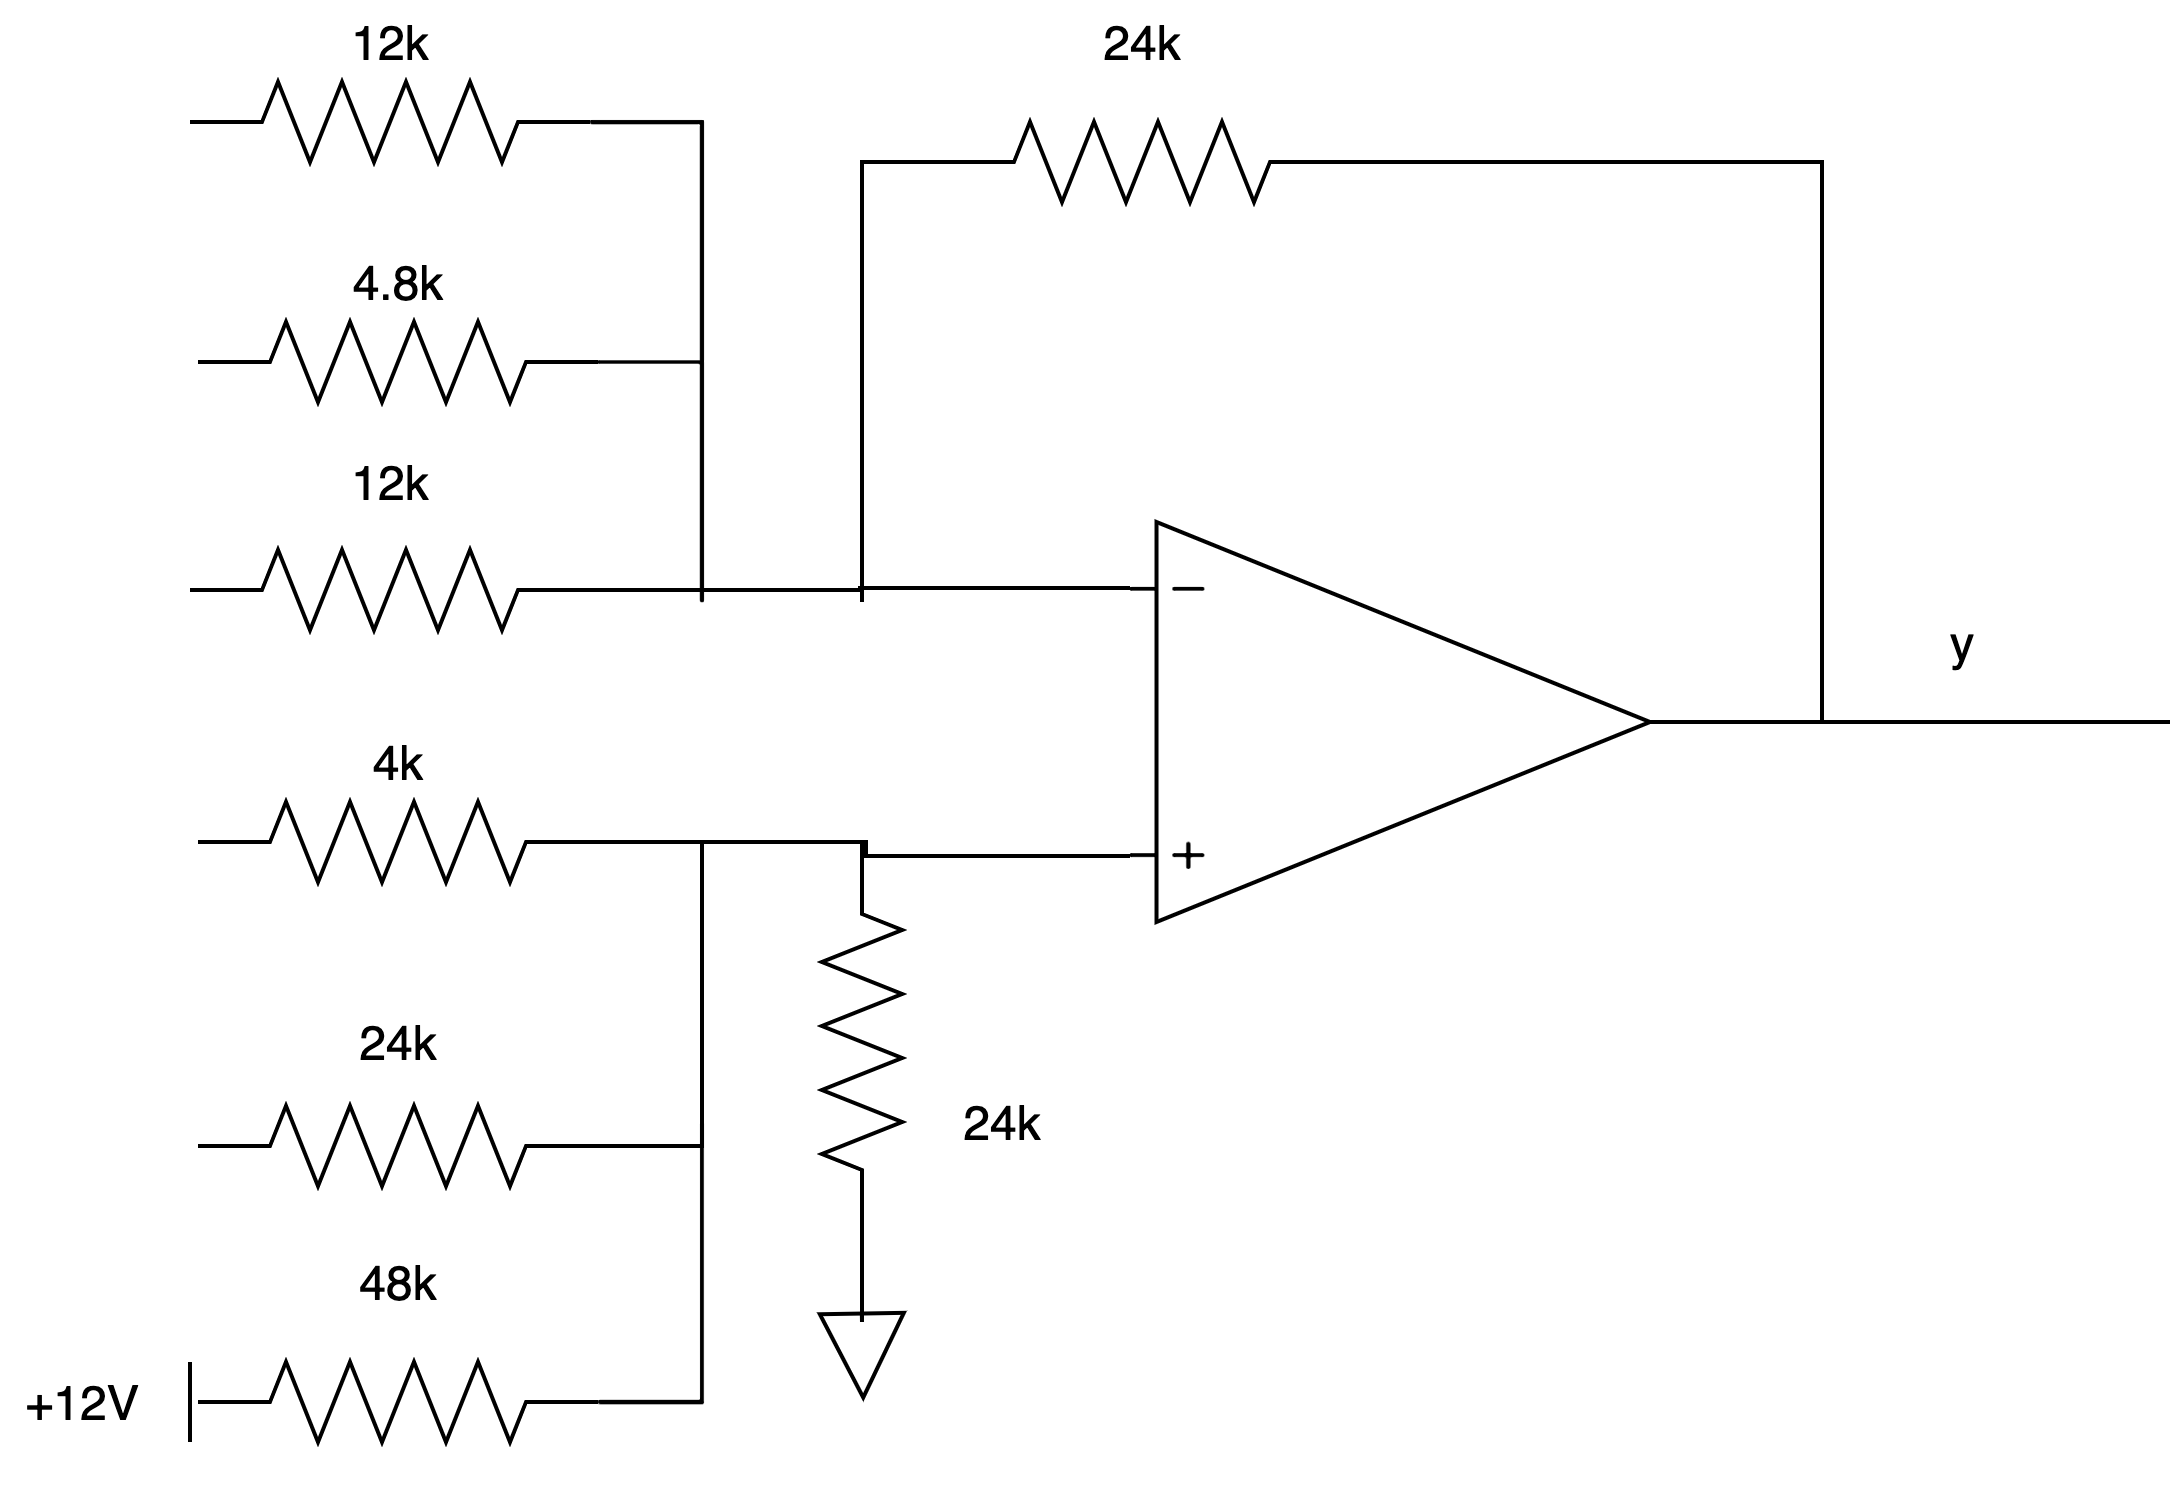
\includegraphics[width=15cm]{circuit.png}
\end{figure}



\end{document}